% !TeX spellcheck = en_GB

\section{Specification}\label{sec:specification}

\subsection{Overview}
Figure \ref{fig:architecture-overview} presents an overview over the Redbackup \gls{system}. All actors, components and interactions are described in detail in the following sections.

\begin{figure}[h]
    \centering
    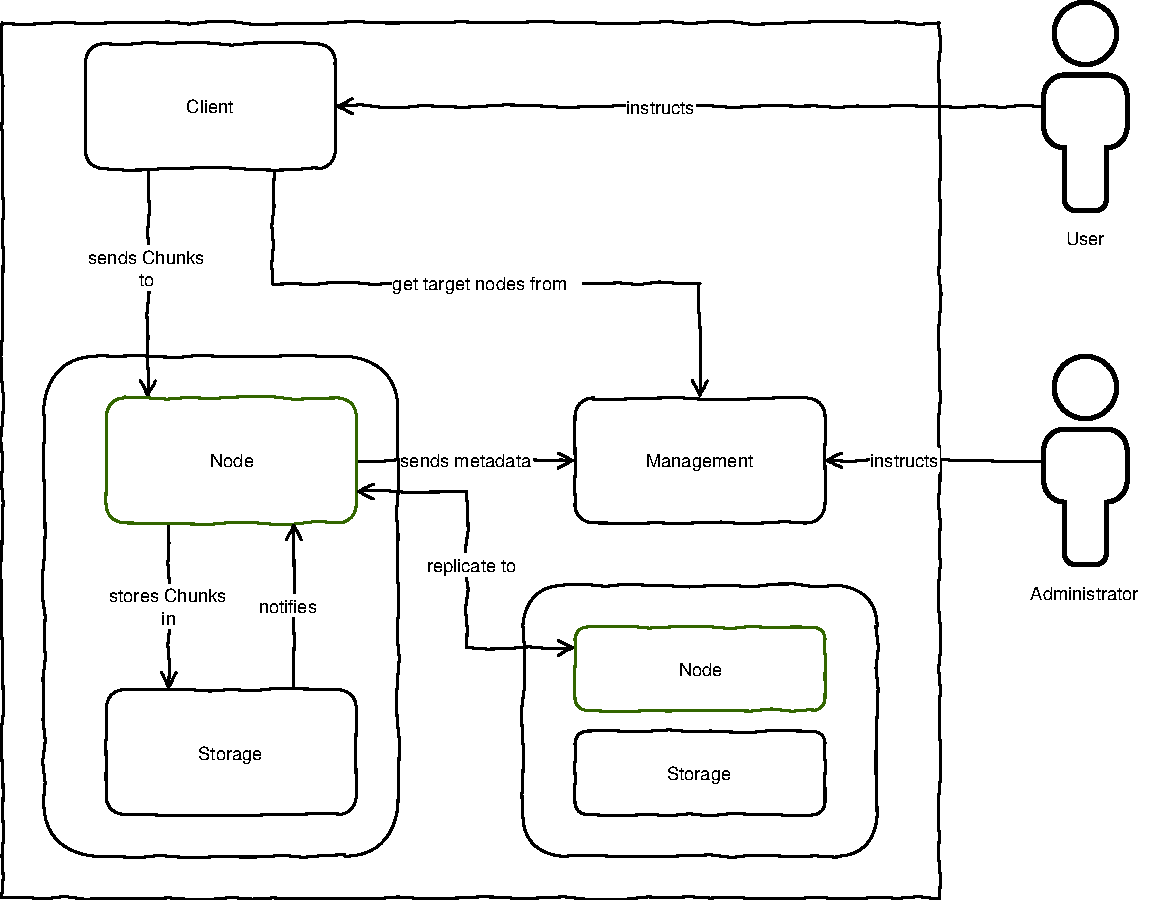
\includegraphics[width=1\linewidth]{resources/architecture_overview}
    \caption{A simplified \gls{system} overview}
    \label{fig:architecture-overview}
\end{figure}

\subsection{Actors}

\subsubsection{User}
A typical \gls{user} does not want to interact with the \gls{system} at any time. All he/she wants is to be sure that all his/her data is backed up.

To simplify the implementation for the study project, the \gls{user} must instruct the \gls{client} manually (create and restore backup).

\paragraph{Responsibilities}
\begin{itemize}
    \item Instruct the \gls{client} to create a Backup
    \item Instruct the \gls{client} to restore a Backup
\end{itemize}


\subsubsection{Administrator}
An \gls{administrator} wants to interact with the \gls{system} as less as possible. He/She wants to be sure that the \gls{system} runs smoothly. If something goes wrong, he/she wants to be able to fix it within a few minutes.

\paragraph{Responsibilities}
\begin{itemize}
    \item Instruct the \gls{management} to add/remove \glspl{node} from the \gls{system}
    \item Ensure that the \gls{management} runs properly (e.g. monitor it)
    \item Act if the \gls{management} notifies him/her about any anomalies
\end{itemize}

\subsection{Components}

\subsubsection{Client}\label{sec:component-client}

\begin{figure}[h]
    \centering
    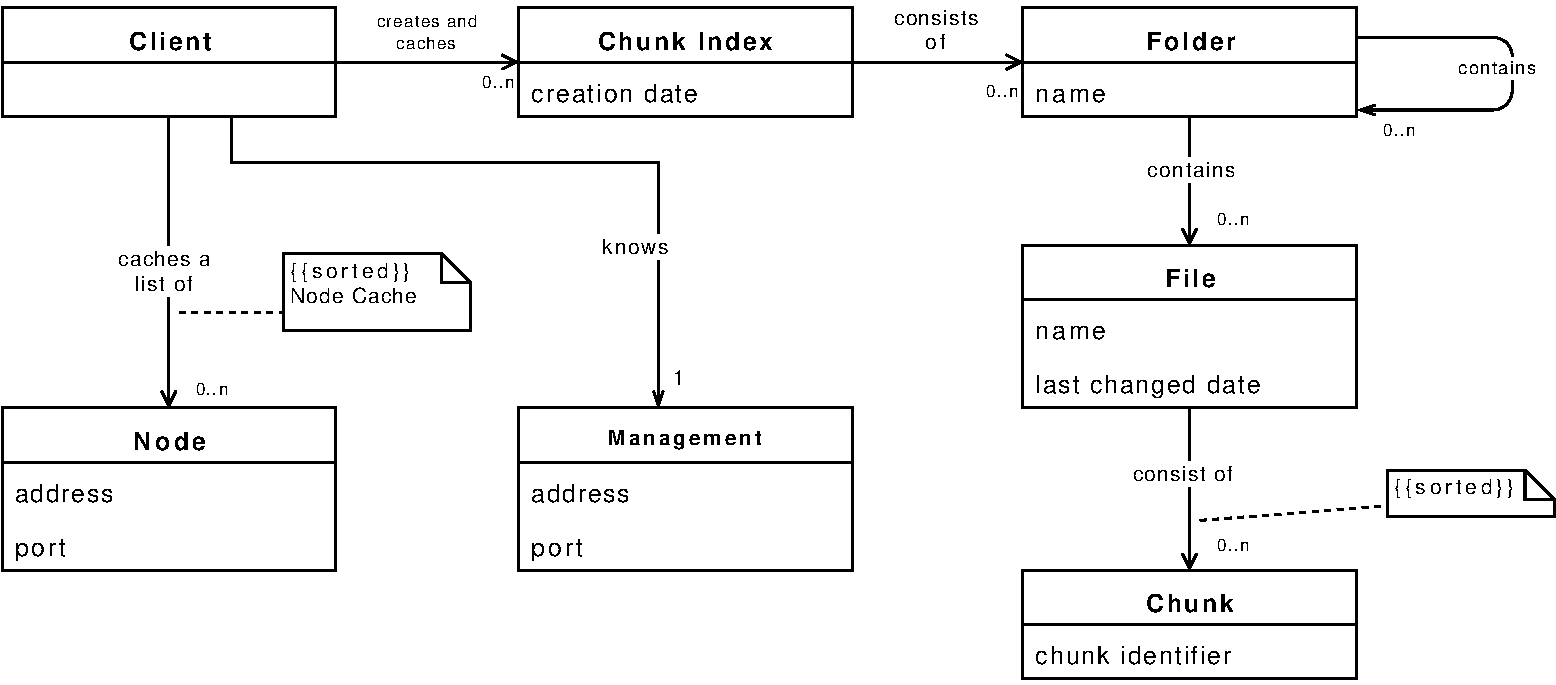
\includegraphics[width=1\linewidth]{resources/client_domain_model}
    \caption[Client Subdomain]{Subdomain illustrating the \glspl{client} perspective}
\end{figure}

\begin{itemize}
    \item The \gls{client} knows the \gls{management} by configuration.
    \item The \gls{client} queries the \gls{management} for a list of \glspl{node}, to which he can send backups or restore previous backups. He caches the results in its \gls{node-cache}.
    \item The \gls{chunk-index} hierarchically models the file system. This structure might change in the future when supporting symlinks and permissions \cite{borg-data-structures}.
    \item The relationship between a given \gls{file} and its \glspl{chunk} is essential. The \gls{client} splits a \gls{file} into multiple \glspl{chunk} to speed up the backup of large data. During the study project, a \gls{file} consists of exactly one \gls{chunk}.
    \item A \gls{chunk} is identified by its \gls{chunk-identifier}, which can be calculated using a hash function which takes the \glspl{chunk-content}  as input.
    \item The \glspl{chunk-content} do not have be present on the \gls{client}. During backup, the \gls{client} can calculate the \glspl{chunk-content} and the corresponding \gls{chunk-identifier} from the \glspl{file} on the disk. On restore, the \gls{client} fetches the \glspl{chunk-content} from a \gls{node} and reassembles the \gls{file} based on the \gls{chunk-index}.
\end{itemize}

% TODO: Serialised Metadata = Serialised version of a given Chunk Index.

\paragraph{Responsibilities}


\begin{itemize}
    \item Keeping the \gls{node-cache} up to date
    \item Create Backups (See Scenario \ref{sec:scenario-create-backup}: \nameref{sec:scenario-create-backup})
    \begin{itemize}
        \item Building/Calculating the \gls{chunk-index}
        \item Serialize the \gls{chunk-index} into \glspl{chunk} including a \gls{root-handle}
        \item Send \glspl{chunk} to \glspl{node}
        \item Mark \glspl{chunk} as \glspl{root-handle}
    \end{itemize}
    \item Restore Backups (See Scenario \ref{sec:scenario-backup-restore}: \nameref{sec:scenario-backup-restore})
    \begin{itemize}
        \item Fetch \glspl{root-handle} from \glspl{node}
        \item Fetch \glspl{chunk} from \glspl{node}
        \item Deserialize \glspl{chunk-index}
        \item Reassemble \glspl{chunk} into \glspl{file} (not required for the study project)
        \item Let the \gls{user} choose which \glspl{file} from which \gls{chunk-index} shall be restored.
    \end{itemize}
\end{itemize}

\subsubsection{Node}\label{sec:component-node}

\begin{figure}[h]
    \centering
    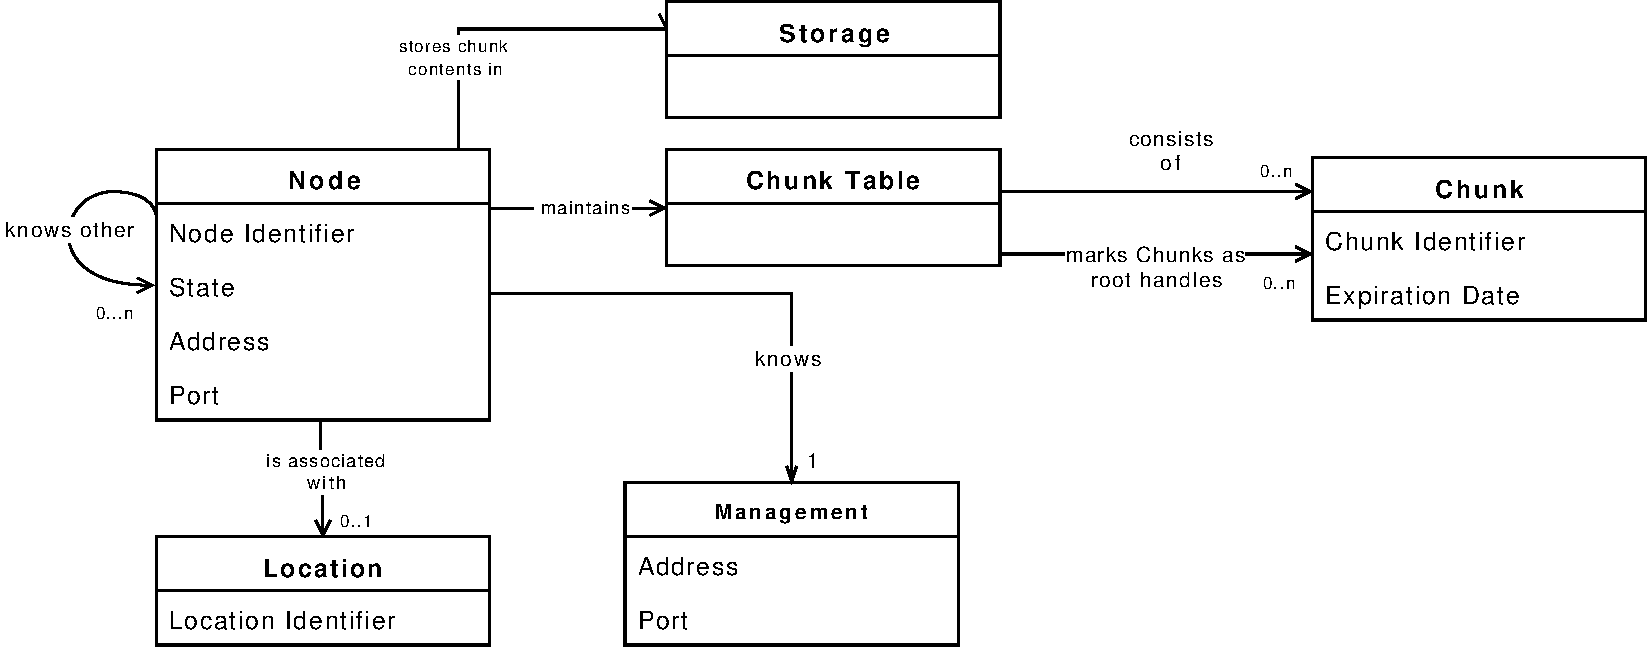
\includegraphics[width=1\linewidth]{resources/node_domain_model}
    \caption[Node Subdomain]{Subdomain illustrating the \glspl{node} perspective}
\end{figure}

\begin{itemize}
    \item A \gls{node} is identified by its unique \gls{node-identifier}. It can be addressed using a certain \emph{Address} and \emph{Port}.
    \item A \gls{node} is also associated with a \gls{location} which will be a replication criteria in the future.
    \item A \gls{node} knows the \gls{management} by configuration and exchanges data with it on a regular basis (Messages \emph{get nodes metadata} and \emph{post nodes metadata})
    \item A \gls{node} is in a given \gls{node-state} and acts differently depending on it (See Figure \ref{fig:node-states}).
    \begin{itemize}
        \item \emph{uninitialized}: The \gls{node} queries the \gls{management} for initialization and does nothing else.
        \item \emph{participating}: This is the "normal" \gls{node-state} in which a \gls{node} accepts backups, performs replication and sends requested data.
        \item \emph{unreachable}: A \gls{node} is marked as \emph{unreachable} if any other \gls{node} or the \gls{management} can not reach it. A \gls{node} never sees itself in this \gls{node-state}.
        \item  \emph{leaving soon}: The \gls{node} does not answer any requests and ensures that all its data is replicated. When it is done, it automatically switches into the \emph{left} \gls{node-state}.
        \item \emph{left}: The \gls{node} has nothing to do in this \gls{node-state} and can shut down.
    \end{itemize}
    \item A \gls{node} knows all other \glspl{node} in the \gls{system} and maintains a \gls{node-state} (see Figure~\ref{fig:node-states}) for them as well.
    \item The \glspl{chunk-content} are stored in a \gls{storage}. See \fullref{sec:component-storage} for further details.
    \item Which \glspl{chunk} are stored on the \gls{node}, their \gls{expiration-date} and the information whether a \gls{chunk} is a \gls{root-handle} is stored in the \gls{chunk-table}.
\end{itemize}

\begin{figure}[h]
    \centering
    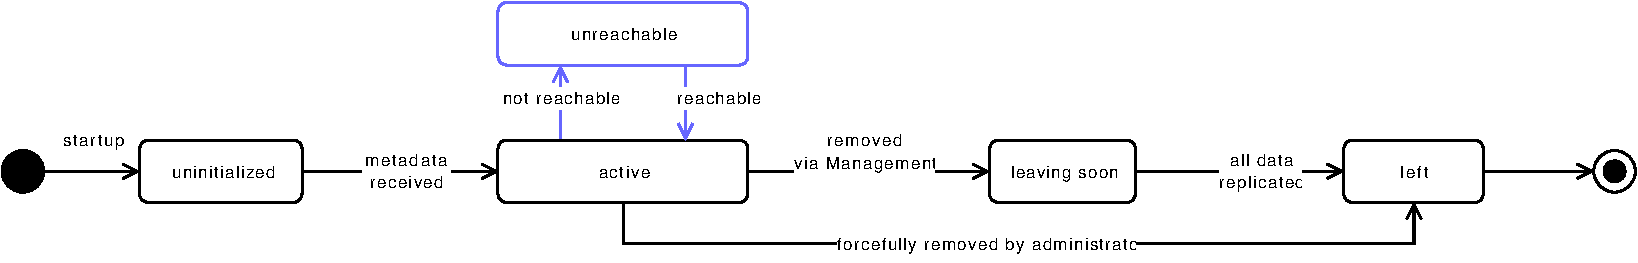
\includegraphics[width=1\linewidth]{resources/node_state}
    \caption[Node States]{A UML State Diagram describing the \glspl{node-state}}
    \label{fig:node-states}
\end{figure}

\paragraph{Responsibilities}

\begin{itemize}
    \item Send \gls{node-metadata} periodically (Messages \emph{get nodes metadata} and \emph{post nodes metadata}) in order to ...
    \begin{itemize}
        \item Perform initialization
        \item Learn about other \glspl{node}
        \item Start the \emph{leaving} process and notify the \gls{management} when it is completed
        \item Send \gls{node-metadata} to the \gls{management} so that it can perform health-checks (e.g. verify the timestamp)
    \end{itemize}
    \item Maintain the \gls{chunk-table}
    \begin{itemize}
        \item Update \glspl{expiration-date}
        \item Add new \glspl{chunk}
        \item Remove expired \glspl{chunk}
    \end{itemize}
    \item Handle possible \gls{storage} issues (see Scenario \ref{sec:scenario-storage-errors} \nameref{sec:scenario-storage-errors})
    \item Reply to \emph{get designation}  (Scenario \ref{sec:scenario-create-backup} \nameref{sec:scenario-create-backup}) , \emph{get root handles} (Scenario \ref{sec:scenario-backup-restore} \nameref{sec:scenario-backup-restore}) and \emph{get chunks} requests
    \item Replicate \glspl{chunk} (See Scenario \ref{sec:scenario-data-replication} \nameref{sec:scenario-data-replication})
    \item Handle \emph{leaving} process (see Scenario \ref{sec:scenario-node-leave-planned} \nameref{sec:scenario-node-leave-planned})
\end{itemize}

\subsubsection{Storage}\label{sec:component-storage}

\begin{figure}[h]
    \centering
    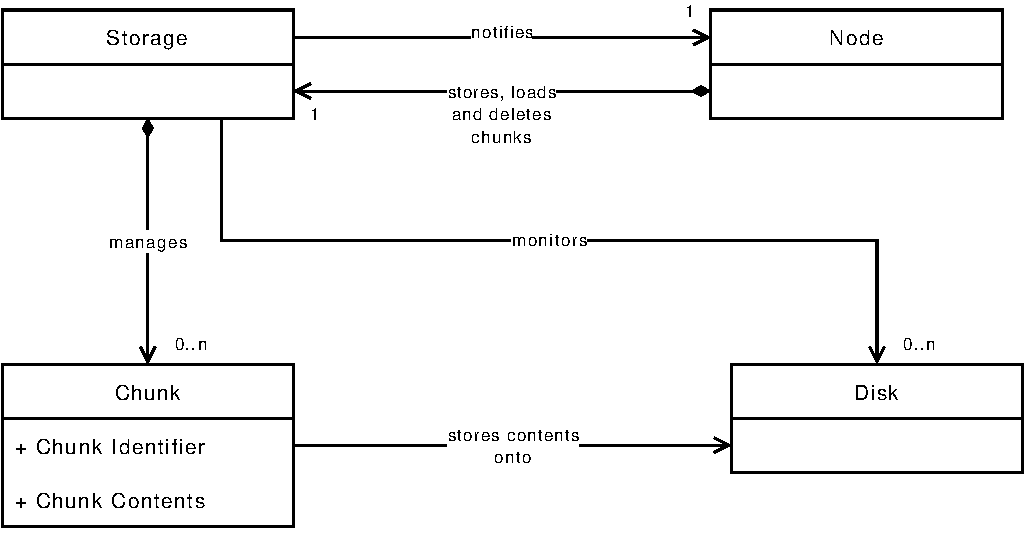
\includegraphics[width=1\linewidth]{resources/storage_domain_model}
    \caption[Storage Subdomain]{Subdomain illustrating the \gls{storage}s perspective}
\end{figure}

\begin{itemize}
    \item The main purpose of the \gls{storage} component is to persist \glspl{chunk-content}. A \gls{storage} is associated with one \gls{node} which stores, loads and deletes \glspl{chunk-content} by its \gls{chunk-identifier} on the \gls{storage}. The same \gls{node} is notified by the \gls{storage} e.g. when corrupted data is detected.
    \item A \gls{chunk} should also monitor the \glspl{medium}, on which the \glspl{chunk-content} are stored, for possible issues and report them to the \gls{node}. This feature, however, is not implemented in the study project.
    \item The \gls{storage} component is deployed on the same host as the \gls{node} that is using it.
\end{itemize}


\paragraph{Responsibilities}

\begin{itemize}
    \item Store \glspl{chunk-content}
    \item Load and return the \glspl{chunk-content} for a given \gls{chunk-identifier}
    \item Delete the \glspl{chunk-content} for a given \gls{chunk-identifier}
    \item Detect possible corruption of \glspl{chunk-content}
    \item Perform service checks on the \glspl{medium} (e.g. S.M.A.R.T tests)
    \item Notify the \gls{node} when a corruption / integrity problem occurs
\end{itemize}

\subsubsection{Management}\label{sec:component-management}

\begin{figure}[h]
    \centering
    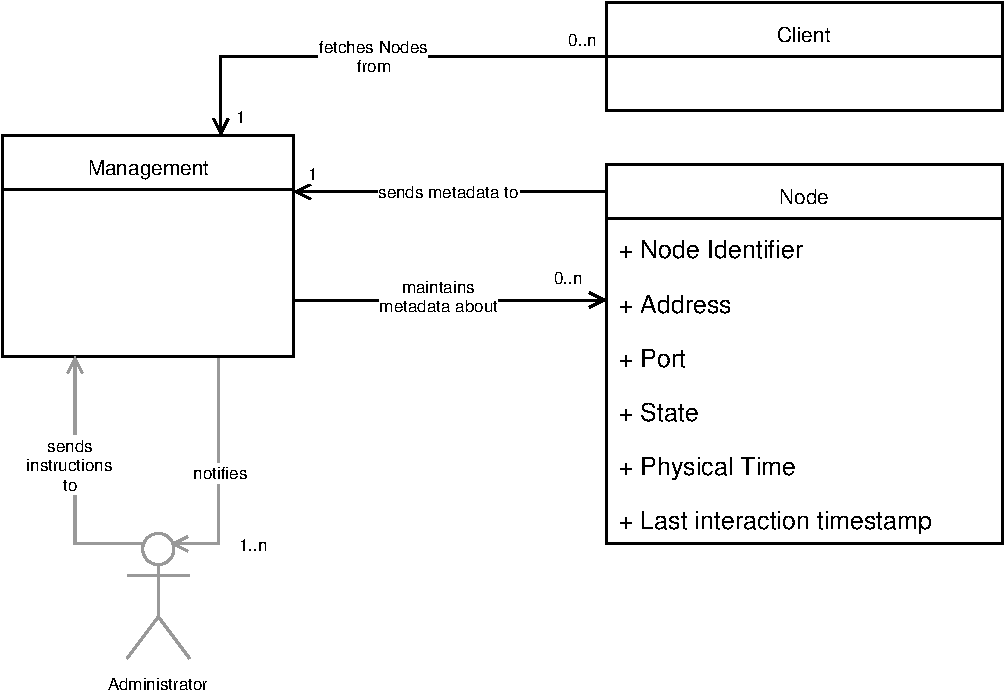
\includegraphics[width=0.75\linewidth]{resources/management_domain_model}
    \caption[Management Subdomain]{Subdomain illustrating the \gls{management}'s perspective}
\end{figure}
\begin{itemize}
    \item The \gls{administrator} is the only Actor interacting with the \gls{management}. He/She sends instructions (e.g. add new \gls{node}) and is notified by the \gls{management} about any anomalies.
    \item \glspl{client} fetch a list of all \glspl{node} from the \gls{management} (See Component \ref{sec:component-client} \nameref{sec:component-client} for further details). As for the study project, the \gls{management} does not have any information about \glspl{client}, but this might change when authentication is implemented in the future.
    \item The \gls{management} maintains \gls{node-metadata} for each \gls{node} in the \gls{system} and sends that information every \gls{node} when they post their \gls{node-metadata}.
\end{itemize}

\paragraph{Responsibilities}
\begin{itemize}
    \item Add and remove \glspl{node}
    \item Notify the \gls{administrator} e.g. if a \gls{node} leaves unexpectedly.
    \item Receive \gls{node-metadata} from the \glspl{node} and reply with \gls{node-metadata}
    \item Send list of \glspl{node} to the \glspl{client}
\end{itemize}

\subsection{Scenarios}
\label{sec:scenarios}
This section describes various scenarios of \gls{system} usage and possible failures.

In the sequence diagrams, we use the composition of the minimal integration test, detailed in Figure \ref{fig:integrationtestsmall} (Chapter \ref{integration-tests}).
The \gls{client} sends its data to \Gls{node} A only.

\subsubsection{Create Backup}\label{sec:scenario-create-backup}
The \gls{client} wants to create a backup.

\begin{figure}[h]
    \centering
    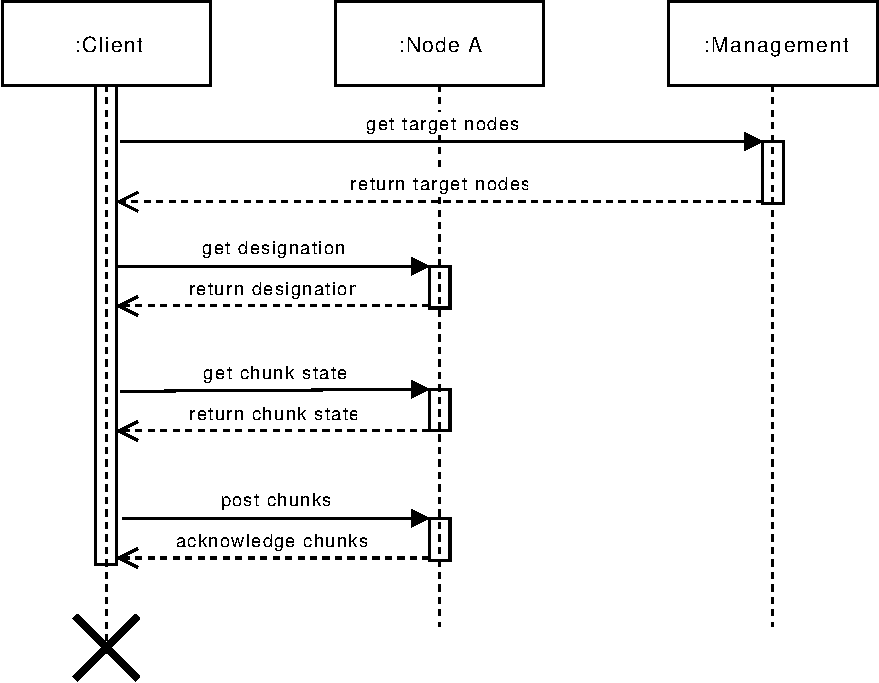
\includegraphics[width=\linewidth]{resources/create_backup}
    \caption{Create Backup Sequence Diagram}
    \label{fig:create-backup}
\end{figure}

\begin{enumerate}
    \item The \gls{client} asks the \gls{management} for a list of \glspl{node}. The \gls{management} returns a sorted list of all \glspl{node} (message: \emph{get target nodes}) (sorting might be based on specific configuration).
        \begin{itemize}
            \item If the \gls{management} is down and this is a first time backup, the \gls{client} records a message and aborts.
            \item If the \gls{management} is down, \gls{client} tries the same \glspl{node} as last time.
        \end{itemize}
    \item The \gls{client} tries to contact \glspl{node} in the presorted order.
        \begin{enumerate}
            \item The \gls{client} sends a backup request (message: \emph{get designation}).
            \item The \gls{node} acknowledges or denies the backup request (message: \emph{return designation}).
            \item If the \gls{node} acknowledges, it is declared as \gls{designated-node}.
            \item If the \gls{node} denies the backup request, the \gls{client} tries the next \gls{node}.
            \item If no \gls{node} answers the request, the \gls{client} records an error message and aborts.
       \end{enumerate}
   \item If the backup request was successful, the \gls{client} starts creating a backup.
        \begin{enumerate}
            \item The \gls{client} splits all \glspl{file} that changed since the last backup into \glspl{chunk-content} and calculate a corresponding hash, the \gls{chunk-identifier} and add it to the local \gls{chunk-index}.
            \item \Glspl{file} that have not changed since the last backup, are already be present in the \gls{chunk-index}.
            \item The \gls{client} send all \glspl{chunk-identifier} present in the \gls{chunk-index} combined with an \gls{expiration-date} to the \gls{designated-node}. (message: \emph{get chunk states})
            \item The \gls{designated-node} checks, if all \glspl{chunk-identifier} received from the \gls{client} are present in its \gls{chunk-table}.
                \begin{itemize}
                    \item If a \gls{chunk-identifier} is already present on the \gls{designated-node}, update its \gls{expiration-date} if it is further in the future.
                    \item If a \gls{chunk-identifier} is not present on the \gls{designated-node}, request it from the \gls{client} (see message response \emph{return chunk states} for further details)
                \end{itemize}
            \item The \gls{client} sends the requested \glspl{chunk-content} to the \gls{designated-node} with a \emph{post chunks} message. %TODO: Abschluss client transaktion (root handle)
                \begin{enumerate}
                    \item The \gls{designated-node} verifies and persists the \glspl{chunk-content} into its \gls{storage}. Afterwards, it acknowledges receipt to the \gls{client} (see \emph{acknowledge chunks} response message).
                                   %TODO: Client must remember, which chunks have been acknowledged. This could be done with a sliding window for QoS/memory usage?
                    \item The \gls{designated-node} replicates \gls{chunk-content} and their \gls{expiration-date} in a continuous replication process. (See scenario~\fullref{sec:scenario-data-replication})
                \end{enumerate}
            \item The \gls{client} serializes its \gls{chunk-index} into a \gls{serialised-chunk-index} and splits it into \glspl{chunk} as well. %TODO: Serialised Metadata is the chunk index plus backup metadata as linked list
            \item The \gls{client} sends the additional \glspl{chunk-content} (as \emph{post chunks} messages) to the \gls{designated-node}, in which the \gls{root-handle} is highlighted. %TODO: The root handle holds a reference to the first list chunk as well as owner etc. information.
        \end{enumerate}
\end{enumerate}

\paragraph{Special cases}
\begin{itemize}
    \item If the \gls{client} is suspended while running, it continuous with the backup process on resume. %TODO: If the expiration date is in the past, the node should refuse the chunk.
    \item If a \gls{file} is changed during the backup process, and the \glspl{chunk-content} and \glspl{chunk-identifier} cannot be calculated, the backup process must be restarted. %TODO: This may lead to starvation.
    \item If \gls{client} crashes, the backup is aborted and won't be continued if the \gls{client} is restarted.
    \item If the \gls{designated-node} goes away (disconnects/crashes/shuts down) during the backup process, the \gls{client} tries to resume the process. After a certain time (e.g. 15m), the \gls{client} gives up and restarts the backup process from the beginning.
    \item A \gls{node} must reject (i.e.\ not acknowledge) \glspl{chunk-content}, if the timestamp of the sending party (e.g. \gls{client}) is e.g.\ an hour in the future or past to prevent data loss on bad synchronized clocks.
    \item If the \gls{designated-node} runs out of storage capacity, it does reject further \glspl{chunk-content}. After a timeout, the \gls{client} restarts the backup process (with another \gls{designated-node}).
\end{itemize}

\paragraph{Possible simplifications in this study project}
\begin{description}
    \item[3a)] Do not split \glspl{file} into \glspl{chunk} but send them as is.
\end{description}

\subsubsection{Backup Restore}\label{sec:scenario-backup-restore}
The \gls{client} wants to restore specific \glspl{file}.

\begin{figure}[h]
    \centering
    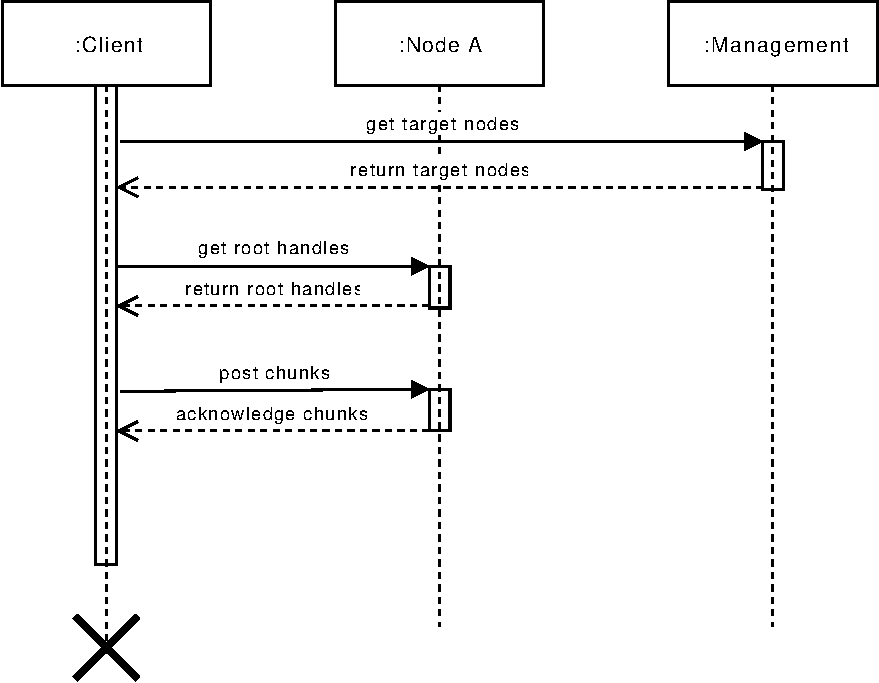
\includegraphics[width=\linewidth]{resources/backup_restore.pdf}
    \caption{Backup Restore Sequence Diagram}
    \label{fig:backup-restore}
\end{figure}

\begin{enumerate}
    \item Same as in scenario~\fullref{sec:scenario-create-backup} step 1.
    \item The \gls{client} contacts the \glspl{node} in the presorted order
        \begin{enumerate}
            \item The \gls{client} sends a \emph{get root handles} requests to a \gls{node}, the \gls{designated-node}.
            \item The \gls{designated-node} returns all \glspl{root-handle} present in the \gls{system} (see \emph{return root handles} message)
            \item If no \gls{node} answers the request,the \gls{client} records an error message and aborts.
        \end{enumerate}
    \item The \gls{client} fetches all \glspl{chunk-content} of the \glspl{serialised-chunk-index} from the \gls{designated-node} (message: \emph{get chunks}) and reassembles the \glspl{chunk-index}.
    \item The \gls{user} specifies which \glspl{file} from which \gls{chunk-index} shall be restored.
    \item The \gls{client} looks up the \glspl{chunk-identifier} in the corresponding \gls{chunk-index}.
    \item The \gls{client} requests the \glspl{chunk-content} from the \gls{designated-node}. (message: \emph{get chunks})
    \item The \gls{client} reassembles the \glspl{chunk-content} into \glspl{file}.
\end{enumerate}

\paragraph{Special cases}
\begin{itemize}
    \item If the \gls{designated-node} does not have a requested \gls{chunk-identifier} in its \gls{chunk-table}, it requests the corresponding \gls{chunk-content} recursively.
    \item If the \gls{client} crashes, the restore process must be repeated
    \item If the \gls{designated-node} is unavailable, the \gls{client} selects a new \gls{designated-node} after a certain timeout (e.g.\ 5m)
\end{itemize}

\paragraph{Possible simplifications in this study project}
\begin{description}
    \item[-] The \gls{client} must request a \gls{node} that has the data already available (possibly the \gls{designated-node}, where the backup was created).
\end{description}


\subsubsection{Node Joining}\label{sec:scenario-node-join}
A \gls{new-node} joins the \gls{system}.

\begin{figure}[h]
    \centering
    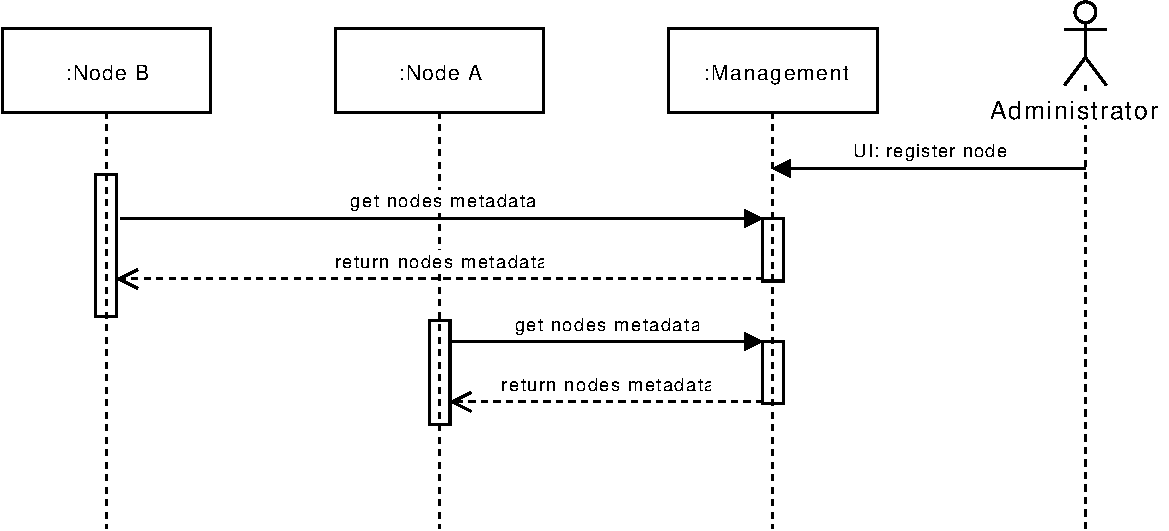
\includegraphics[width=\linewidth]{resources/node_joining.pdf}
    \caption{Node Joining Sequence Diagram}
    \label{fig:node-joining}
\end{figure}

This scenario is described as it is implemented in the study project. It might be subject to further evaluation in the future.

\begin{enumerate}
    \item The \gls{new-node} is registered by an \gls{administrator} in the \gls{management} using its \gls{node-identifier}. A \gls{location} must also be assigned to the \gls{node}. %TODO: Data
    \item The \gls{new-node} queries \gls{node-metadata} from the \gls{management} (message: \emph{get nodes metadata}) on startup.
    \item The \gls{new-node} configures itself based on its \gls{node-identifier} and received \gls{node-metadata} from \gls{management}.
        \begin{itemize}
            \item If the \gls{management} has no information available (yet) or is unavailable, the \gls{new-node} retries after a certain timeout (e.g.\ 5min).
        \end{itemize}
    \item Other \glspl{node} learn about the \gls{new-node} through periodical \gls{node-metadata} queries (message: \emph{post nodes metadata})
        \begin{enumerate}
            \item If the \gls{new-node} contacts an existing \gls{node}, before the existing \gls{node} updates its \gls{node-metadata}, the existing \gls{node} should query the \gls{management} (message: \emph{get nodes metadata})
            \item If the \gls{management} is unavailable, the \gls{new-node} ignores all communication attempts.
        \end{enumerate}
\end{enumerate}

\subsubsection{Node Leaving Planned}\label{sec:scenario-node-leave-planned}
A \gls{node} leaves the \gls{system} planned (refered as \gls{leaving-node}).

\begin{figure}[h]
    \centering
    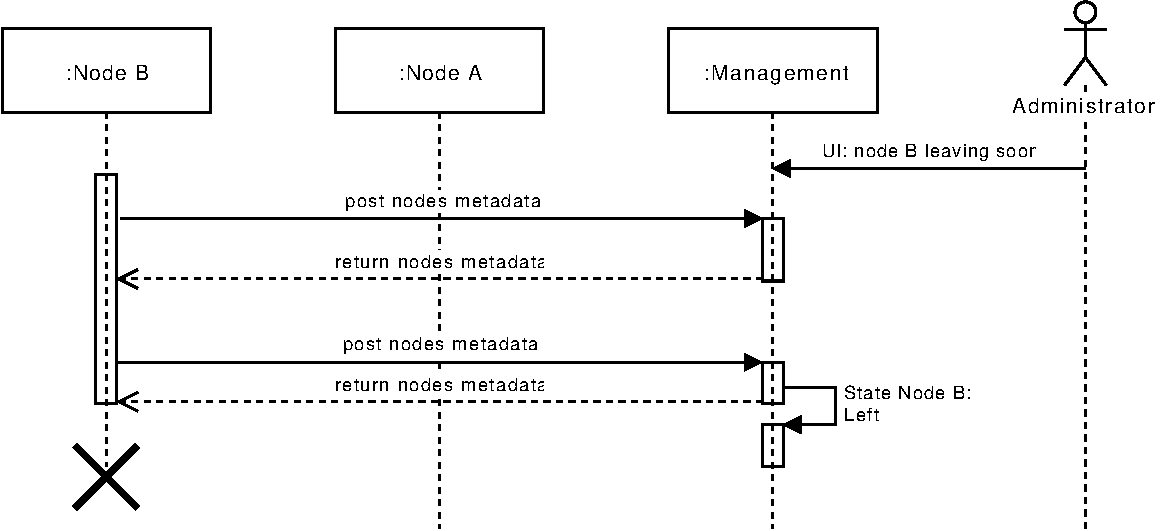
\includegraphics[width=\linewidth]{resources/node_leaving_planned.pdf}
    \caption{Node Leaving Planned Sequence Diagram}
    \label{fig:node-leave-planned}
\end{figure}

This scenario is described as it is implemented in the study project. It might be subject to further evaluation in the future.

\begin{enumerate}
    \item The \gls{leaving-node} is marked as \emph{leaving soon} by the \gls{administrator} in the \gls{management}.
    \item As soon as the \gls{leaving-node} realises that it is in \gls{node-state} \emph{leaving soon} (using \emph{post nodes metadata}), it ignores messages from other \glspl{node}, rejects any new backups and starts replicating its \glspl{chunk-content} to another \gls{node}.
    \item As soon as all \glspl{chunk-content} are replicated onto other \glspl{node}, the \gls{leaving-node} changes its \gls{node-state} to \emph{left} and informs the \gls{management} (message: \emph{post nodes metadata}).
\end{enumerate}

\subsubsection{Node Leaving Unplanned}\label{sec:scenario-node-leave-unplanned}
A \gls{node} leaves the \gls{system} unexpectedly.

\begin{figure}[h]
    \centering
    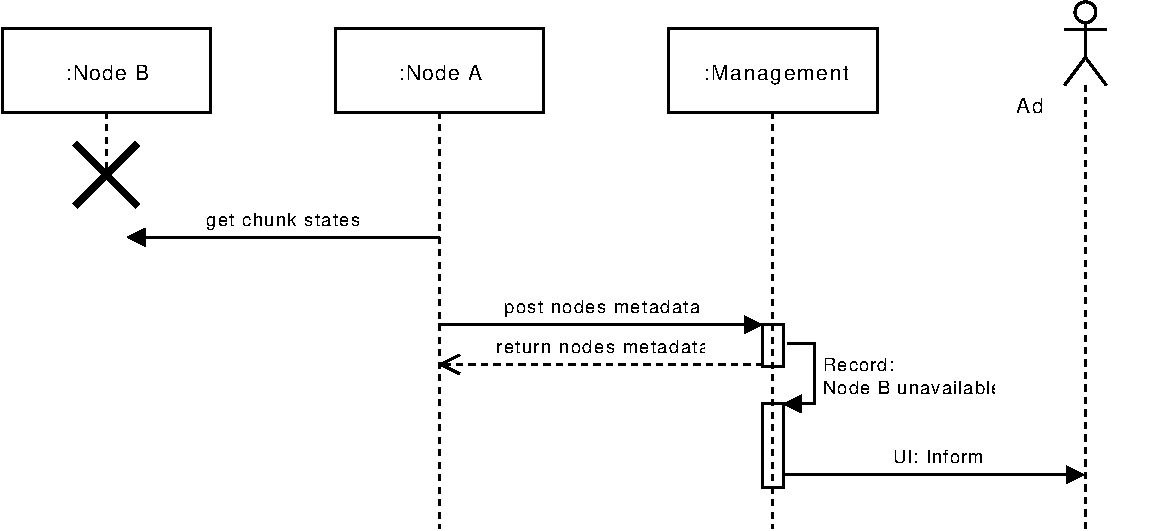
\includegraphics[width=\linewidth]{resources/node_leaving_unplanned.pdf}
    \caption{Node Leaving Unplanned Sequence Diagram}
    \label{fig:node-leave-unplanned}
\end{figure}

This scenario is described as it is implemented in the study project. It might be subject to further evaluation in the future.

\begin{enumerate}
    \item If a \gls{node} is not responding (which means, no other \gls{node} nor the \gls{management} can reach it), the \gls{management} records the unavailability and informs the \gls{administrator}.
    %Replikationsmechanismus; management knows, that on reason of intervall the node is away
\end{enumerate}

\begin{itemize}
    \item If the \gls{node} returns, it carries on as if nothing happend.
    \item If the \gls{node} does not return, the \gls{administrator} marks the \gls{node} as \emph{left}, which is propagated to all \glspl{node} via the \emph{post nodes metadata} message.
        \begin{itemize}
            \item \glspl{chunk-content}, which were not previously replicated from the \gls{node} are lost.
        \end{itemize}
\end{itemize}

\subsubsection{Data Replication}\label{sec:scenario-data-replication}
The network distributes \glspl{chunk}.

\begin{figure}[h]
    \centering
    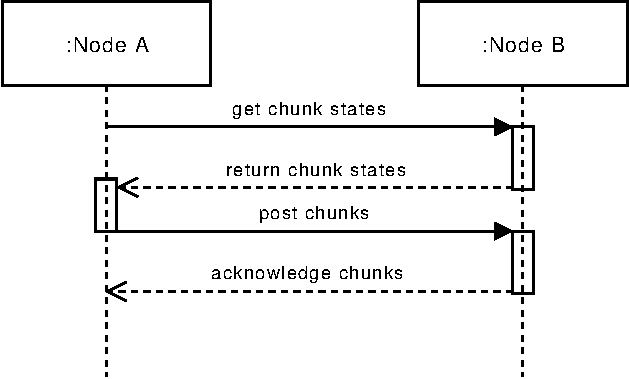
\includegraphics[width=0.6\linewidth]{resources/data_replication.pdf}
    \caption{Data Replication Sequence Diagram}
    \label{fig:data-replication}
\end{figure}

This scenario is described as it is implemented in the study project. It might be subject to further evaluation in the future.

\begin{enumerate}
    \item The \gls{sending-node} picks $n$ random entries from its \gls{chunk-table}. In the future, these entries might be selected based on heuristics.
    \item The \gls{sending-node} picks one random \gls{designated-node} from its \gls{node-metadata}. In the future, the \gls{designated-node} might be selected based on heuristics.
    \item The \gls{sending-node} sends the \glspl{chunk-identifier} of the chosen entries to the \gls{designated-node} with a \emph{get chunk states} message.
    \item The \gls{designated-node} checks, if all \glspl{chunk-identifier} received from the \gls{sending-node} are present in its \gls{chunk-table}.
        \begin{itemize}
            \item If a \gls{chunk-identifier} is already present, update its \gls{expiration-date} if it is further in the future.
            \item If a \gls{chunk-identifier} is not present, request the corresponding \gls{chunk-content} from the \gls{sending-node} (see message \emph{return chunk states} for further details).
        \end{itemize}
    \item The \gls{sending-node} sends the requested \glspl{chunk-content} to the \gls{designated-node} with a \emph{post chunks} message.
        \begin{itemize}
            \item The \gls{designated-node} verifies and persists the \glspl{chunk-content} into its \gls{storage}. Afterwards, it acknowledges receipt to the \gls{sending-node} (see \emph{acknowledge chunks} response message).
        \end{itemize}
\end{enumerate}

\subsubsection{Data has Expired Lifetime}\label{sec:scenario-data-expiration}
A \gls{node} wants to delete \glspl{chunk} with a past \gls{expiration-date}.

This scenario is described as it is implemented in the study project. It might be subject to further evaluation in the future.

\begin{itemize}
    \item The \gls{management} monitors the \glspl{node} physical timestamp and records any deviation from the \gls{management} time larger than 1h.
    \item Therefore, a first prototype, the \gls{node} may just delete \glspl{chunk} after the specified \gls{expiration-date} without further checks.
        \begin{itemize}
            \item We build on the assumption, that the \glspl{node} have different upstream timeservers, so that a general time shift is unlikely.
            \item In case a single \gls{node}s time is in the past, and runs out of storage capacity, it might lead to a redundancy loss.
            \item If a single \gls{node}s time is in the future, the redundancy is reduced by one.
        \end{itemize}
\end{itemize}

In the future, it is advisable to implement a consent protocol to reduce the likelihood of data loss.

\subsubsection{Data Storage has Errors}\label{sec:scenario-storage-errors}
The \gls{storage} component notifies its \gls{node} that a \gls{chunk} stored in it is corrupt.

This scenario is described as it is implemented in the study project. It might be subject to further evaluation in the future.

\begin{enumerate}
    \item The \gls{storage} informs the \gls{node} of a corrupt \gls{chunk} using its \gls{chunk-identifier}
    \item The \gls{node} removes the \gls{chunk-identifier} from the \gls{chunk-table}
        \begin{itemize}
            \item The \gls{chunk} will be replicated eventually.
        \end{itemize}
    \item Inform \gls{management} when sending the next \emph{post nodes metadata} message.
\end{enumerate}

\subsubsection{Management Problems}\label{sec:scenario-management-problems}
\begin{itemize}
    \item The case that the \gls{management} has outdated \gls{node-metadata} due to data loss will be ignored during this study project.
\end{itemize}

\subsubsection{Network Availability Problems}\label{sec:scenario-network-errors}
\paragraph{Behaviour in case a node can reach only some nodes directly}
The still available \glspl{node} should try to satisfy redundancy needs as good as possible.
If a \gls{node} cannot reach other \glspl{node}, it notifies the \gls{management} with the next \emph{post nodes metadata}

\paragraph{Behaviour in case the network gets partitioned}
(, and the \glspl{node} in each partition can only reach each other and not the other ones.)

See first case in scenario~\fullref{sec:scenario-network-errors}

\paragraph{Behaviour in case nodes have different states of management information}
The redundancy is temporary reduced to the \glspl{node} which the group of old \glspl{node} know, but will eventually be resolved as \glspl{node} fetch \gls{node-metadata}.


\subsection{Messages}\label{sec:messages}

\Glspl{message} denote the communication units between application components. The following message specification is not bound to a specific message format (e.g. BSON or Protobuf) on purpose since it might change in the future to optimise performance.

A \gls{message} is separated into a \gls{message-header} and \gls{message-payload} section. In the future, the \gls{message-header} section might get extended by e.g. a \texttt{message size} and \texttt{checksums}.

\begin{figure}[h]
    \centering
    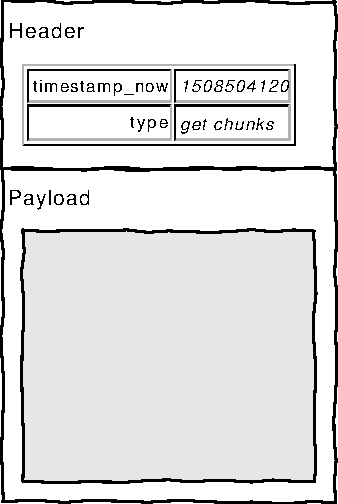
\includegraphics[width=0.3\linewidth]{resources/message_schematic}
    \caption[\Gls{message} Schematic]{Schematic of a \gls{message}}
    \label{fig:messageschematic}
\end{figure}

\begin{table}[H]
    \begin{tabu}{| >{\ttfamily}l | X |}
        \hline
        header
        & Set of \glspl{header-field} elements as specified in Table \ref{tab:message-field-header}. \\
        
        \hline
        payload
        & The actual payload of the message depending on the message type defined in the \gls{header-field} \texttt{type} (see Table \ref{tab:core-header-fields}). \\

        \hline
    \end{tabu}
    \caption[\Gls{message} Structure]{Structure of a \gls{message}.}
    \label{tab:message}
\end{table}

\begin{table}[H]
\begin{tabu}{| >{\ttfamily}l | X |}
    \hline
    field name
    & Unique name of the \gls{header-field}. A core set of \gls{header-field} that must be sent with every request is defined in Table \ref{tab:core-header-fields}. \\
    
    \hline
    field value
    & The value belonging to the field name. \\

    \hline
\end{tabu}
\caption{Structure of a \gls{header-field} element}
\label{tab:message-field-header}
\end{table}


\begin{table}[H]
    \begin{tabu}{| >{\ttfamily}l | X |}
        \hline
        timestamp\_now
        & The current UTC time of the local clock as a unix timestamp (64-bit).  \\
        
        \hline
        type
        & A string representation of the message type, as described in subsections \fullref{sec:messages}. \\
        \hline
    \end{tabu}
    \caption{Core set of \glspl{header-field} sent with every request}
    \label{tab:core-header-fields}
\end{table}

\subsubsection{get target nodes}\label{sec:get-target-nodes}

\begin{table}[H]
    \begin{tabu}{lX}
        Context
        & \makecell[tl]{
            \fullref{sec:scenario-create-backup} \\
            \fullref{sec:scenario-backup-restore}
          } \\
        
        Sender
        & A \gls{client} \\
        
        Receiver
        & The \gls{management} \\
        
        Additional message headers
        &  No additional \glspl{message-header} required \\
        
        Message payload
        & The \gls{message-payload} is empty \\

        Response
        & \fullref{sec:return-target-nodes} (compulsory) \\
    \end{tabu}
    \caption{\texttt{get target nodes} message specification}
\end{table}

\subsubsection{return target nodes}\label{sec:return-target-nodes}
\begin{table}[H]
    \begin{tabu}{lX}
        Context
        & Response to \fullref{sec:get-target-nodes} \\
        
        Sender
        & The \gls{management} \\
        
        Receiver
        & The \gls{client} that sent the \texttt{get target nodes} message \\
        
        Additional message headers
        &  No additional \glspl{message-header} required \\
        
        Message payload
        & See Table \ref{tab:payload-return-target-nodes}\\

        Response
        & No response \\
    \end{tabu}
    \caption{\texttt{return target nodes} message specification}
\end{table}


\begin{table}[H]
    \begin{tabu}{| >{\ttfamily}l | X |}
        \hline
        target\_nodes
            & A list of \texttt{target node elements} as defined in Table \ref{tab:element-target-nodes}. The list is sorted in descending order by preference. \\
        \hline
    \end{tabu}
    \caption{Structure of the \texttt{return target nodes} \gls{message-payload}}
    \label{tab:payload-return-target-nodes}
\end{table}

\begin{table}[H]
    \begin{tabu}{| >{\ttfamily}l | X |}
        \hline
        node\_identifier
        & \Gls{node-identifier} of the \gls{node}. \\
        
        \hline
        address
        &  Address (domain name or IP) of the \gls{node}. \\
        
        \hline
        port
        &  Port-Number of the \gls{node}. \\

        \hline
    \end{tabu}
    \caption{Structure of the \texttt{target node element}}
    \label{tab:element-target-nodes}
\end{table}

\subsubsection{get designation}\label{sec:get-designation}

\begin{table}[H]
    \begin{tabu}{lX}
        Context
        & \fullref{sec:scenario-create-backup} \\
        
        Sender
        & A \gls{client} \\
        
        Receiver
        & A \gls{node} \\
        
        Additional message headers
        &  No additional \glspl{message-header} required \\
        
        Message payload
        & See Table \ref{tab:message-get-designation} \\

        Response
        & \fullref{sec:return-designation} (compulsory) \\
    \end{tabu}
    \caption{\texttt{get designation} message specification}
\end{table}

\begin{table}[H]
    \begin{tabu}{| >{\ttfamily}l | X |}
        \hline
        estimate\_size
        & Backup size estimate by the \gls{client} in bytes. \\
        
        \hline
        expiration\_date
        & Unix timestamp (64-bit) of UTC timezone, until when the backup is scheduled to be kept.\\
        
        \hline
    \end{tabu}
    \caption{Structure of the \emph{get designation} \gls{message-payload}.}
    \label{tab:message-get-designation}
\end{table}

\subsubsection{return designation}\label{sec:return-designation}
\begin{table}[H]
    \begin{tabu}{lX}
        Context
        & Response to \fullref{sec:get-designation} \\
        
        Sender
        & The \gls{node} that received the \texttt{get designation} message  \\
        
        Receiver
        & The \gls{client} that sent the \texttt{get designation} message \\
        
        Additional message headers
        &  No additional \glspl{message-header} required \\
        
        Message payload
        & See Table \ref{tab:message-return-designation}\\

        Response
        & No response \\
    \end{tabu}
    \caption{\texttt{return designation} message specification}
\end{table}

\begin{table}[H]
    \begin{tabu}{| >{\ttfamily}l | X |}
        \hline
        designation
        & Boolean, whether or not the node is ready to receive the backup. \\
        \hline
    \end{tabu}
    \caption{Structure of the \emph{return designation} \gls{message-payload}.}
    \label{tab:message-return-designation}
\end{table}

\subsubsection{get chunk states}\label{sec:get-chunk-states}
\begin{table}[H]
    \begin{tabu}{lX}
        Context
        & \makecell[tl]{
            \fullref{sec:scenario-create-backup} \\
            \fullref{sec:scenario-data-replication}
          } \\
        
        Sender
        & A \gls{client} or a \gls{node} \\
        
        Receiver
        & A \gls{node} \\
        
        Additional message headers
        &  No additional \glspl{message-header} required \\
        
        Message payload
        & See Table \ref{tab:message-get-chunk-states}\\

        Response
        & \fullref{sec:return-chunk-states} (compulsory) \\
    \end{tabu}
    \caption{\texttt{get chunk states} message specification}
\end{table}

\begin{table}[H]
    \begin{tabu}{| >{\ttfamily}l | X |}
        \hline
        chunks
        & A set of \texttt{chunk elements} as defined in Table \ref{tab:chunk-element} for which the state shall be checked. \\
        \hline
    \end{tabu}
    \caption{Structure of the \texttt{get chunk states} \gls{message-payload}}    
    \label{tab:message-get-chunk-states}
\end{table}

\begin{table}[H]
    \begin{tabu}{| >{\ttfamily}l | X |}
        \hline
        chunk\_identifier
        & The \gls{chunk-identifier} of this \gls{chunk}\\
        
        \hline
        expiration\_date
        & The \gls{expiration-date} of this \gls{chunk} \\

        \hline        
        root\_handle
        & Boolean, whether this \gls{chunk} is a \gls{root-handle} \\

        \hline
    \end{tabu}
    \caption{Structure of the \texttt{chunk element}}
    \label{tab:chunk-element}
\end{table}

\subsubsection{return chunk states}\label{sec:return-chunk-states}

\begin{table}[H]
    \begin{tabu}{lX}
        Context
        & Response to \fullref{sec:get-chunk-states} \\
        
        Sender
        & The \gls{node} that received the \texttt{get chunk states} message\\
        
        Receiver
        & The \gls{client} or \gls{node} that sent the \texttt{get chunk states} message \\
        
        Additional message headers
        &  No additional \glspl{message-header} required \\
        
        Message payload
        & See Table \ref{tab:message-return-chunk-states}\\

        Response
        & No response \\
    \end{tabu}
    \caption{\texttt{return chunk states} message specification}
\end{table}

\begin{table}[H]
    \begin{tabu}{| >{\ttfamily}l | X |}
        \hline
        chunks
        & A set of \texttt{chunk elements} as defined in Table \ref{tab:chunk-element} that are present on this node with the updated \texttt{expiration\_date} \\
        \hline
    \end{tabu}
    \caption{Structure of the \texttt{return chunk states} \gls{message-payload}}    
    \label{tab:message-return-chunk-states}
\end{table}

\subsubsection{post chunks}\label{sec:post-chunks}

\begin{table}[H]
    \begin{tabu}{lX}
        Context
        & \makecell[tl]{
            \fullref{sec:scenario-create-backup} \\
            \fullref{sec:scenario-data-replication}
          } \\
        
        Sender
        & A \gls{client} or a \gls{node} \\
        
        Receiver
        & A \gls{node} \\
        
        Additional message headers
        &  No additional \glspl{message-header} required \\
        
        Message payload
        & See Table \ref{tab:message-post-chunks}\\

        Response
        & \fullref{sec:acknowledge-chunks} (compulsory) \\
    \end{tabu}
    \caption{\texttt{post chunks} message specification}
\end{table}

\begin{table}[H]
    \begin{tabu}{| >{\ttfamily}l | X |}
        \hline
        chunks
        & A set of \texttt{chunk content elements} as defined in Table \ref{tab:chunks-content-element}. \\
        \hline
    \end{tabu}
    \caption{Structure of the \texttt{post chunks} \gls{message-payload}}
    \label{tab:message-post-chunks}
\end{table}

\begin{table}[H]
    \begin{tabu}{| >{\ttfamily}l | X |}
        \hline
        chunk\_identifier
        & The \gls{chunk-identifier} of this \gls{chunk}\\
        
        \hline
        expiration\_date
        & The \gls{expiration-date} of this \gls{chunk} \\

        \hline        
        root\_handle
        & Boolean, whether this \gls{chunk} is a \gls{root-handle} \\

        \hline
        chunk\_content
        & The binary \glspl{chunk-content} of this \gls{chunk} \\
        \hline
    \end{tabu}
    \caption{Structure of the \texttt{chunk content element}}
    \label{tab:chunks-content-element}
\end{table}

\subsubsection{acknowledge chunks}\label{sec:acknowledge-chunks}

\begin{table}[H]
    \begin{tabu}{lX}
        Context
        & Response to \fullref{sec:post-chunks} \\
        
        Sender
        & The \gls{node} that received the \texttt{post chunks} message\\
        
        Receiver
        & The \gls{client} or \gls{node} that sent the \texttt{post chunks} message \\
        
        Additional message headers
        &  No additional \glspl{message-header} required \\
        
        Message payload
        & See Table \ref{tab:message-acknowledge-chunks}\\

        Response
        & No response \\
    \end{tabu}
    \caption{\texttt{acknowledge chunks} message specification}
\end{table}

\begin{table}[H]
    \begin{tabu}{| >{\ttfamily}l | X |}
        \hline
        chunks
        &  A set of \texttt{chunk elements} as defined in Table \ref{tab:chunk-element} that were received and stored. \\
        \hline
    \end{tabu}
    \caption{Structure of the \texttt{acknowledge chunks} \gls{message-payload}}    
    \label{tab:message-acknowledge-chunks}
\end{table}


\subsubsection{get chunks}\label{sec:get-chunks}
\begin{table}[H]
    \begin{tabu}{lX}
        Context
        & \fullref{sec:scenario-backup-restore} \\
        
        Sender
        & A \gls{client} \\
        
        Receiver
        & A \gls{node} \\
        
        Additional message headers
        &  No additional \glspl{message-header} required \\
        
        Message payload
        &  See Table \ref{tab:message-get-chunks}\\

        Response
        & \fullref{sec:return-chunks} (compulsory) \\
    \end{tabu}
    \caption{\texttt{get chunks} message specification}
\end{table}

\begin{table}[H]
    \begin{tabu}{| >{\ttfamily}l | X |}
        \hline
        chunk\_identifiers
        & A set of \glspl{chunk-identifier} for which the \glspl{chunk-content} shall be returned. \\
        \hline    
    \end{tabu}
    \caption{Structure of the \texttt{get chunks} \gls{message-payload}}
    \label{tab:message-get-chunks}
\end{table}

\subsubsection{return chunks}\label{sec:return-chunks}
\begin{table}[H]
    \begin{tabu}{lX}
        Context
        & Response to \fullref{sec:get-chunks} \\
        
        Sender
        & The \gls{node} that received the \texttt{get chunks} message \\
        
        Receiver
        & The \gls{client} that sent the \texttt{get chunks} message \\
        
        Additional message headers
        &  No additional \glspl{message-header} required \\
        
        Message payload
        & See Table \ref{tab:message-return-chunks}\\

        Response
        & No response \\
    \end{tabu}
    \caption{\texttt{return chunks} message specification}
\end{table}

\begin{table}[H]
    \begin{tabu}{| >{\ttfamily}l | X |}
        \hline
        chunks
        & A set of \texttt{chunk content elements} as defined in Table \ref{tab:chunks-content-element}. \\
        \hline
    \end{tabu}
    \caption{Structure of the \texttt{return chunks} \gls{message-payload}}    
    \label{tab:message-return-chunks}
\end{table}



\subsubsection{get root handles}\label{sec:get-root-handles}
\begin{table}[H]
    \begin{tabu}{lX}
        Context
        & \fullref{sec:scenario-backup-restore} \\
        
        Sender
        & A \gls{client} \\
        
        Receiver
        & A \gls{node} \\
        
        Additional message headers
        &  No additional \glspl{message-header} required \\
        
        Message payload
        & The \gls{message-payload} is empty. \\

        Response
        & \fullref{sec:return-root-handles} (compulsory) \\
    \end{tabu}
    \caption{\texttt{get root handles} message specification}
\end{table}

\subsubsection{return root handles}\label{sec:return-root-handles}
\begin{table}[H]
    \begin{tabu}{lX}
        Context
        & Response to \fullref{sec:get-root-handles} \\
        
        Sender
        & The \gls{node} that received the \texttt{get root handles} message \\
        
        Receiver
        & The \gls{client} that sent the \texttt{get root handles} message \\
        
        Additional message headers
        &  No additional \glspl{message-header} required \\
        
        Message payload
        & See Table \ref{tab:message-return-root-handles}\\

        Response
        & No response \\
    \end{tabu}
    \caption{\texttt{return root handles} message specification}
\end{table}

\begin{table}[H]
    \begin{tabu}{| >{\ttfamily}l | X |}
        \hline
        root\_handle\_chunks
        & A set of \texttt{chunk content elements} as defined in Table \ref{tab:chunks-content-element}, all of which are \glspl{root-handle} \\
        \hline
    \end{tabu}
    \caption{Structure of the \texttt{return root handles} \gls{message-payload}}
    \label{tab:message-return-root-handles}
\end{table}


\subsubsection{get nodes metadata}\label{sec:get-nodes-metadata}

\begin{table}[H]
    \begin{tabu}{lX}
        Context
        & \makecell[tl]{
            \fullref{sec:scenario-node-join} \\
            Periodical \gls{node} updates: \gls{node} reads data from \gls{management} only
          } \\
        
        Sender
        & A \gls{node} \\
        
        Receiver
        & The \gls{management} \\
        
        Additional message headers
        &  No additional \glspl{message-header} required \\
        
        Message payload
        & The \gls{message-payload} is empty. \\

        Response
        & \fullref{sec:return-nodes-metadata} (compulsory) \\
    \end{tabu}
    \caption{\texttt{get nodes metadata} message specification}
\end{table}

\subsubsection{post nodes metadata}\label{sec:post-nodes-metadata}
\begin{table}[H]
    \begin{tabu}{lX}
        Context
        & \makecell[tl]{
            \fullref{sec:scenario-node-join} \\
            Periodical \gls{node} updates: Node sends data
          } \\
        
        Sender
        & A \gls{node} \\
        
        Receiver
        & The \gls{management} \\
        
        Additional message headers
        &  No additional \glspl{message-header} required \\
        
        Message payload
        &  See Table \ref{tab:message-post-nodes-metadata}\\
        
        Response
        & \fullref{sec:return-nodes-metadata} (compulsory) \\
    \end{tabu}
    \caption{\texttt{post nodes metadata} message specification}
\end{table}

\begin{table}[H]
    \begin{tabu}{| >{\ttfamily}l | X |}
        \hline
        this\_node
        & An \texttt{internal node metadata element} as described in Table \ref{tab:internal-node-metadata-element} describing the sending \gls{node}. \\
        
        \hline
        other\_nodes
        & A set of \texttt{node state metadata elements} as described in Table \ref{tab:node-state-metadata-element}. One element for for every other \gls{node} in the \gls{system} about which the sending \gls{node} is aware of.\\
        \hline
    \end{tabu}
    \caption{Structure of the \texttt{post nodes metadata} \gls{message-payload}}
    \label{tab:message-post-nodes-metadata}
\end{table}

\begin{table}[H]
    \begin{tabu}{| >{\ttfamily}l | X |}
        \hline
        node\_identifier
        & The \gls{node-identifier} of this \gls{node}\\

        \hline
        state
        & The inner \gls{node-state} of this \gls{node}\\
        
        \hline
        storage\_used
        & Free \gls{storage} of this \gls{node} in \emph{bytes} . \\

        \hline
        storage\_total
        & Total \gls{storage} capacity of this \gls{node} in \emph{bytes}. \\
        \hline
    \end{tabu}
    \caption{Structure of the \texttt{internal node metadata element}}
    \label{tab:internal-node-metadata-element}
\end{table}

\begin{table}[H]
    \begin{tabu}{| >{\ttfamily}l | X |}
        \hline
        node\_identifier
        & The \gls{node-identifier} of this \gls{node}\\

        \hline
        state
        & The \gls{node-state} of this \gls{node} (as seen from the outside)\\
        \hline
    \end{tabu}
    \caption{Structure of the \texttt{node state metadata element}}
    \label{tab:node-state-metadata-element}
\end{table}


\subsubsection{return nodes metadata}\label{sec:return-nodes-metadata}

\begin{table}[H]
    \begin{tabu}{lX}
        Context
        & \makecell[tl]{
            Response to \fullref{sec:post-nodes-metadata} \\
            Response to \fullref{sec:get-nodes-metadata}
          } \\
        
        Sender
        & The \gls{management} \\
        
        Receiver
        & The \gls{node} that sent the \texttt{post nodes metadata} / \texttt{get nodes metadata}  message \\
        
        Additional message headers
        &  No additional \glspl{message-header} required \\
        
        Message payload
        & See Table \ref{tab:message-return-nodes-metadata}\\

        Response
        & No response \\
    \end{tabu}
    \caption{\texttt{return nodes metadata} message specification}
\end{table}


\begin{table}[H]
    \begin{tabu}{| >{\ttfamily}l | X |}
        \hline
        nodes
        & A set of \texttt{node contact metadata elements} as described in Table \ref{tab:node-contact-metadata-element}. One element for for every \gls{node} in the \gls{system}. \\
        \hline
    \end{tabu}
    \caption{Structure of the \texttt{return nodes metadata} \gls{message-payload}}
    \label{tab:message-return-nodes-metadata}
\end{table}
\begin{table}[H]
    \begin{tabu}{| >{\ttfamily}l | X |}
        \hline
        node\_identifier
        & The \gls{node-identifier} of this \gls{node}. \\
        
        \hline
        address
        & The address of this \gls{node}. \\
        
        \hline
        port
        & The \glspl{node} port of this \gls{node}. \\
        
        \hline
        state
        & The \gls{node-state} of this \gls{node}.\\
        \hline
    \end{tabu}
    \caption{Structure of the \texttt{node contact metadata element}}
    \label{tab:node-contact-metadata-element}    
\end{table}